\documentclass[12pt, a4paper]{article}
\usepackage{../notesheets}
%%%%%%%%%%%%%%%%%%%%%%%%%%%%%%%%%%%%%%%%%%%%%%%%%%
\author{Math 1220}
\title{Notesheet. Section 6.5: Evaluation of Definite Integrals}
\date{}

\begin{document}
\maketitle
\nameline
%%%%%%%%%%%%%%%%%%%%%%%%%%%%%%%%%%%%%%%%%%%%%%%%%%
Recall the following:
\begin{defi}
  \begin{enumerate}
  \item We define the \de{indefinite integral} of \(f(x)\) to be \[
      \int f(x) \dx = 
    \]
  \item We define the \de{definite integral} from \(a\) to \(b\) of
    \(f(x)\) to be \[
      \int_a^b f(x) \dx =
    \]
    Note, if \(f(x) \geq 0\), then \(\int_a^b f(x) \dx = \)
  \end{enumerate}
\end{defi}
\begin{thrm}
  \begin{enumerate}
  \item (Fundamental Theorem of Calculus)   If \(f\) is continuous on
    \([a,b]\), then \[
    \int_a^b f(x) \dx = 
  \]
  where \(F\) is any antiderivative of \(f\). 
  \item (Net Change Theorem) If \(f\) is differentiable on \((a,b)\)
    and \(f'\) is continuous on \((a,b)\), then \[
      \int_a^b f'(x) \dx = 
    \]
  \item (Average Value Formula) The average value of integrable
    function \(f\) on \([a,b]\) is given by 
  \end{enumerate}
\end{thrm}
\begin{ex}
  Compute the following indefinite integrals
  \begin{enumerate}
  \item \(\int (2e^x+4\cos x \dx)\)
    \vspace{0.5in}
  \item \(\int x \sin(\sin x) \dx\)
        \vspace{0.5in}
  \item \(\int \frac{\sin(\ln x)}{x} \dx\)
  \end{enumerate}
\end{ex}
\vspace{-1in}
\begin{ex}
  What is the average value of \(f(x) = \cos x\) on \(\left[-\frac{\pi}{2}, \frac{\pi}{2}\right]\)?
\end{ex}
\begin{ex}
  Using geometric reasoning, what is the area of the region bounded
  above by \(f(x) = 1\) on \([0,1]\) and bounded below by \(g(x) = x\)
  on \([0,1]\). Express this area as a combination of definite integrals.
  \\
  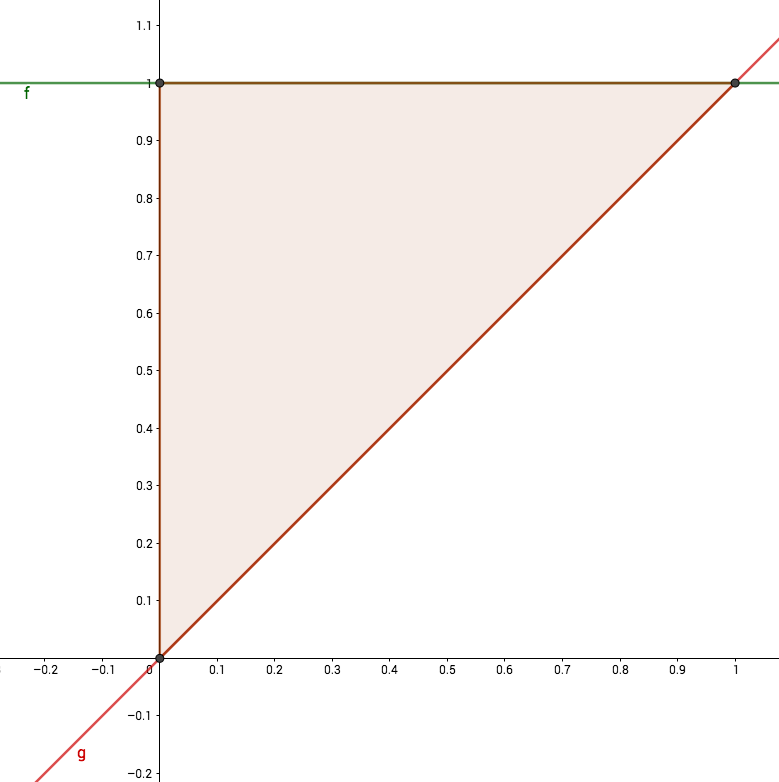
\includegraphics[scale=0.3]{images/region-1}
\end{ex}
%%%%%%%%%%%%%%%%%%%%%%%%%%%%%%%%%%%%%%%%%%%%%%%%%% 
\end{document}
